%!TEX root = ../thesis.tex

\chapter[discussion]{Discussion}\label{chp:discussion}
% ~5 pages
%
% OUTLINE:
% - paper-hierarchical:
%   - Suitability of VAEs for representation learning (minimization of mutual information and sensitivity to implicit prior such as architecture)
% - paper-benchmarking
%   - Inferiority of probabilistic methods compared to self-supervised learning. 
% - 


\section{\Cref{chp:paper-hierarchical} revisited: \dots}

\lesstodo[inline]{Discuss sensitivity to ``implicit" prior such as architecture (and probably optimization method and other). Include reference to \parencite{huszar_is_2017} discussing the usefulness of using a maximum likelihood objective for representation learning in generative models.}
\lesstodo[inline]{Discuss whether VAEs are even suitable for representation learning due to them minimizing a mutual information term in the ELBO (derive this form).}
\lesstodo[inline]{Discuss some recent work e.g. \cref{morningstar_density_2021}}


\section{\Cref{chp:paper-benchmarking} revisited: Bested?}

\lesstodo[inline]{Discuss whether variational autoencoders are viable for learning good representations for speech for downstream tasks when alternatives such as SSL method exist.}
\lesstodo[inline]{Out-of-distribution detection on speech?}


\section{\Cref{chp:paper-review} revisited: \dots} \label{sec:discussion-paper-review}

\lesstodo[inline]{Are self-supervised speech representations useful for unsupervised uncertainty estimation? \parencite{nava_stateconsistency_2021, nava_uncertaintyaware_2021} Within robotics but not really related.}
% Since the main focus within self-supervised learning has been on improving downstream task performance, very limited work, if any, has investigated self-supervised representations in terms of uncertainty estimation. 
% However, in the context of medical applications where data can be abundant but labels are sparse, unsupervised uncertainty estimation is a very interesting direction for future work.
\lesstodo[inline]{OOD data: Generalization or detection (https://arxiv.org/pdf/2110.11334.pdf)?}


\section{\Cref{chp:paper-retrospective} revisited: Calibration}
The work in \textcite{wenstrup_retrospective_2023} focuses on the predictive performance of the ensemble model and an analysis of feature importance, but does not explicitly consider uncertainty estimation. 
As we discussed in \cref{subsec:model-calibration}, such a model can be calibrated to predict probabilities that are aligned with the empirical probability of the model being correct on some validation set.

In \cref{fig_discussion:retrospective-paper-calibration-curve-of-uncalibrated-model}, we plot the calibration curve for the uncalibrated stroke recognition ensemble and the individual models along with a histogram of its predicted probabilities. 
The calibration curve is computed by sorting the predicted probabilities on test set into a number of bins spanning the range from zero to one. For each bin, we compute the fraction of examples for which the model predicted correctly and then plot these pairs of mean predicted probabilities and correctness fractions. A perfectly calibrated model would have the same fraction of correct predictions in any given bin, as that bin's mean value. \Cref{fig_discussion:retrospective-paper-calibration-curve-of-uncalibrated-model} clearly shows the miscalibration issue that we previously discussed. 
It is interesting to note that the ensemble model is better calibrated than the individual models that form it. Since an ensemble output probability is computed as the harmonic mean of the five individual model probabilities, it is easy to see that the ensembles output probability can never exceed the maximum probability predicted among the individual models. This property tends to make ensemble probabilities less extreme and, since the individual models are overconfident, this results in better calibration (see also the histogram in \cref{fig_discussion:retrospective-paper-calibration-curve-of-uncalibrated-model}). 

To calibrate the ensemble model, we can use methods such as Platt-scaling \parencite{platt_probabilistic_1999} or isotonic regression \parencite{zadrozny_transforming_2002}. 
In both cases, we fit a simple regression model (logistic or isotonic) to the predicted probabilities and the target labels on some validation set. 
In \cref{fig_discussion:retrospective-paper-calibration-curve-sigmoid-isotonic} we have done so for the ensemble model using our validation set for fitting and visualizing the results on the test set. On the left, we plot the resulting calibration curves and on the right we show the logistic and isotonic fits. We see that both methods result in quite good calibrations\footnote{Test set Brier scores: Uncalibrated = $0.003500$, logistic = $0.001807$, isotonic = $0.001774$. Brier skill score compared to uncalibrated (relative improvement): Logistic = $0.4830$, isotonic = $0.4924$.} and that the predicted probabilities are shifted towards smaller values. 

While correct calibration provides some interpretability to the predictions, the actual values of the probabilities are still tied of the model's performance. For example, with the logistic calibration, we can note that the predicted probabilities have been shifted so far towards smaller values that the highest possible predicted probability is about 50\%. This means strokes can be predicted at best with a 50\% chance of being correct. 
If this model were to be deployed in a randomized controlled trial, the calibrated probabilities might be incorporated in the design of the user interface such that a user can discern between confident and uncertain model predictions. However, it is easy to imagine how this generally low confidence might lead the user to ignore the model. This highlights a problem with uncertainties

% Brier scores:  {'uncalibrated': 0.0034955788687128925, 'logistic': 0.0018072483306197486, 'isotonic': 0.0017744177396100578, 'average': 0.0021955477869598783}
% BSS uncalibrated reference:  {'logistic': 0.48299025755205005, 'isotonic': 0.4923822902432705}
% BSS mean reference:  {'logistic': 0.17685766561145932, 'isotonic': 0.1918109229282361}

\begin{figure}
    \begin{subfigure}[c]{0.48\columnwidth}
        \centering
        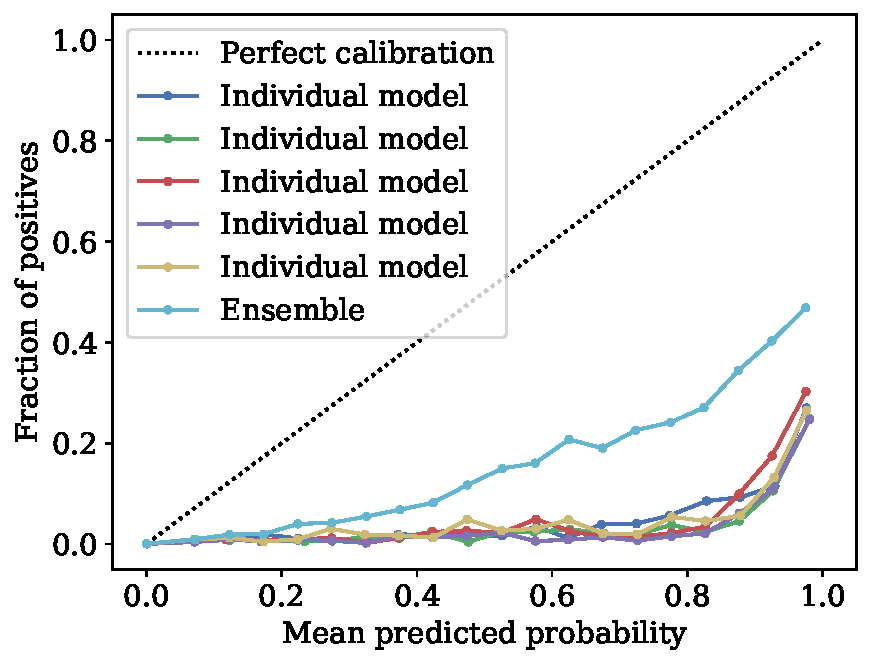
\includegraphics[width=1\columnwidth]{python_plotting/calibration_curve_ensemble_and_all_models_uncalibrated.pdf}
        % \caption{}
        % \label{fig_discussion:calibration_curve_ensemble_and_all_models_uncalibrated}
    \end{subfigure}
    % \hfill
    \begin{subfigure}[c]{0.48\columnwidth}
        \centering
        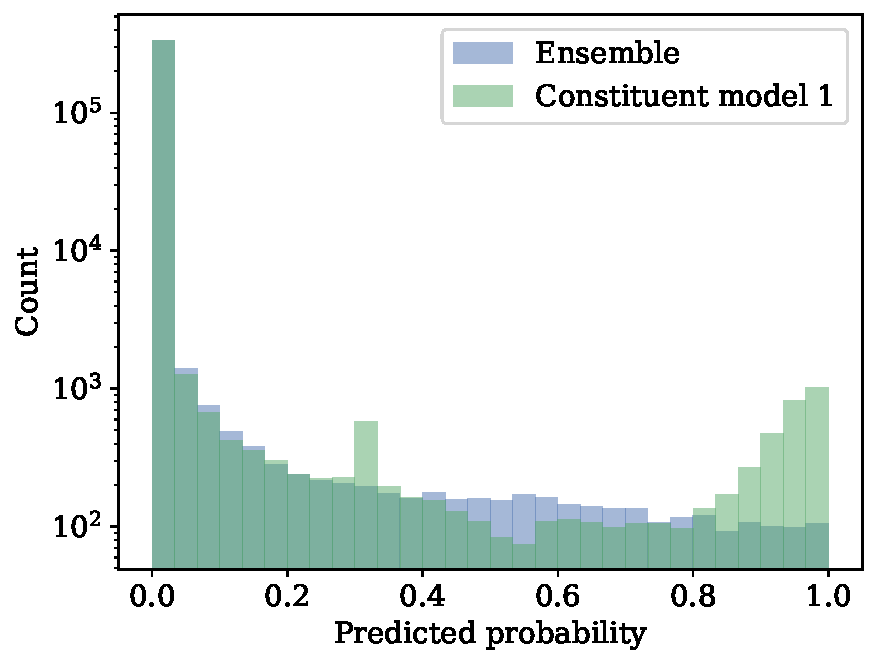
\includegraphics[width=1\columnwidth]{python_plotting/histogram_ensemble_and_single_model.pdf}
        % \caption{}
        % \label{fig_discussion:histogram_ensemble_and_single_model}
    \end{subfigure}
    \caption[Calibration curve for the uncalibrated stroke recognition model and empirical distribution of predicted probabilities.]{%
        Calibration curve for the uncalibrated stroke recognition ensemble model (left) and the histogram of predicted probabilities (right). 
        We use the ensemble that achieved the median F1-score which is the one also reported in \cref{tab_retrospective:table3-occlusion-analysis, fig_retrospective:figure1-roc-curve}.
    }
    \label{fig_discussion:retrospective-paper-calibration-curve-of-uncalibrated-model}
\end{figure}

\begin{figure}
    \begin{subfigure}[c]{0.48\columnwidth}
        \centering
        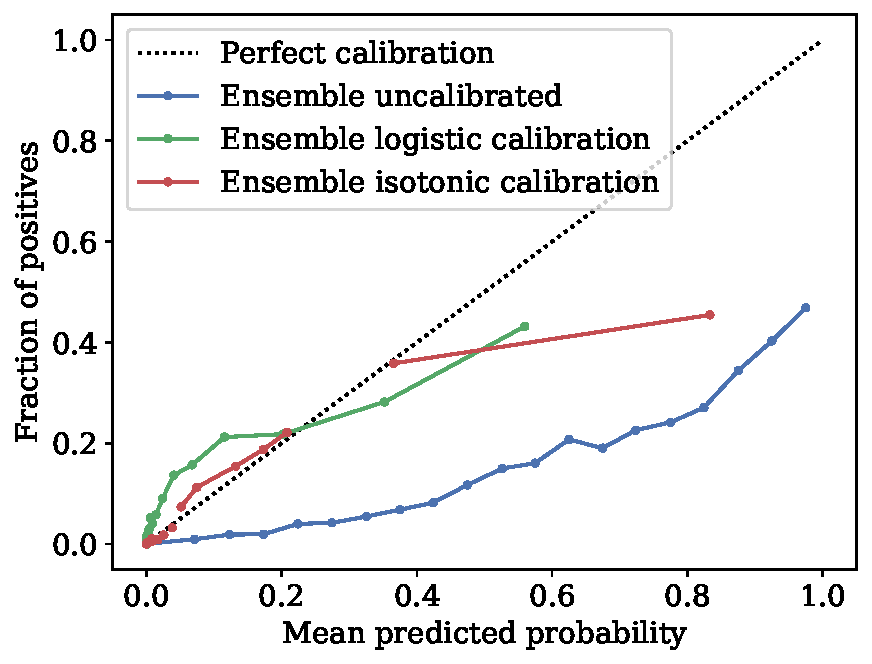
\includegraphics[width=1\columnwidth]{python_plotting/calibration_curves_ensemble.pdf}
        % \caption{}
        % \label{fig_discussion:calibration_curve_ensemble_and_all_models_uncalibrated}
    \end{subfigure}
    % \hfill
    \begin{subfigure}[c]{0.48\columnwidth}
        \centering
        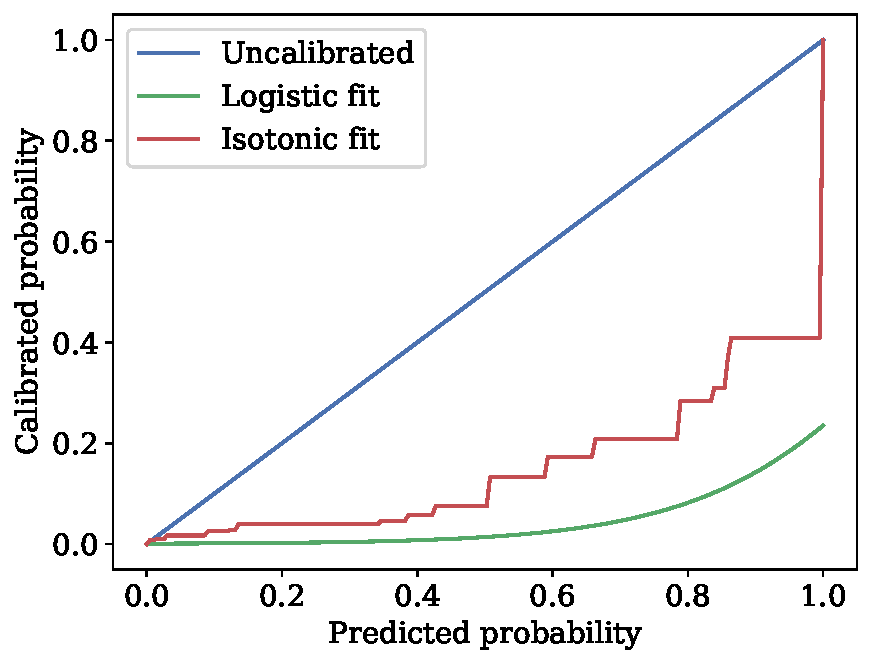
\includegraphics[width=1\columnwidth]{python_plotting/calibration_fits_ensemble.pdf}
        % \caption{}
        % \label{fig_discussion:histogram_ensemble_and_single_model}
    \end{subfigure}
    \caption[Calibration fits and curves for the stroke recognition model using Platt-scaling and isotonic regression for calibration.]{%
        Calibration curves using sigmoid and isotonic calibration fits for the stroke recognition ensemble model (left) and the calibration fits (right). 
        We use the ensemble that achieved the median F1-score which is the one also reported in \cref{tab_retrospective:table3-occlusion-analysis, fig_retrospective:figure1-roc-curve}.
    }
    \label{fig_discussion:retrospective-paper-calibration-curve-sigmoid-isotonic}
\end{figure}


% \subsectionP{Ensembling technique}
% To form an ensemble from several models, we need a method to form a single prediction from the outputs of the individual models.
% To allow us to evaluate an impact score for each word feature in our ablation study, we wanted our ensemble to provide not only predictions but also associated probability scores on a continuous scale. A majority voting scheme would only provide as many different scores as models, in our case five, which is arguably too coarse a resolution. 






\lesstodo[inline]{Discuss the calibration of the stroke model and report calibration curve.}
\lesstodo[inline]{Report the results of calibrating the stroke model using e.g. Platt scaling or Isotonic scaling.} % https://scikit-learn.org/stable/modules/calibration.html


% \lesstodo[inline]{Maybe mention MultiQT paper \parencite{havtorn_multiqt_2020}.}
